\subsection{Classification performance metrics}

\subsubsection{Receiver operating characteristic curve}

To compare the performance of different models, it is common practice to compare their receiver operating characteristic (ROC) curve.
The true positive rate, $TPR = \frac{\text{true positives}}{\text{true positives} + \text{fales negatives}} = TP / (TP + FN)$, is plotted against the false positive rate, $FPR = \frac{\text{false positives}}{\text{false positives} + \text{true negatives}} = FP / (FP + TN)$, at different thresholds for a prediction score to be counted as positive or negative.
The ROC curve always starts at (0, 0) and ends at (1, 1).
The diagonal shows the values above which a classifier performs better than a classifier with an accuracy of 0.5, where accuracy is
\begin{align}
    ACC = \frac{TP + TN}{TP + TN + FP + FN}.
\end{align}
This, however, is not the baseline to beat in the case of an imbalanced dataset.
The always positive classifier has an accuracy that depends on the fraction of positive examples in the dataset $\pi$.
The corresponding baseline is determined by the function
\begin{align}
    TPR = \frac{1 - \pi}{\pi} FPR + 2 - \frac{1}{\pi},
\end{align}
see [ref appendix] for a derivation.
A perfect classifier has an ROC curve that goes from (0, 0) to (0, 1) to (1, 1), such that the area under the ROC curve (AUROC) is the highest.

\subsubsection{Precision-Recall curve}
The ROC curve is not well-suited for imbalanced datasets~\cite{Takaya2015}.
Another way to visualize model performance is plotting precision, $\mathrm{prec} = TP / (TP + FP)$, against $TPR$ (recall, rec), at different thresholds for a prediction score.
The Precision-Recall (PR) curve ignores true negatives and always starts at (0, 1) and ends at (1, 0).
The random classifier has its baseline at $\mathrm{prec} = \pi$.
The baseline of the always positive classifier is the point where $\mathrm{rec} = 1$ and $\mathrm{prec = \pi}$.

Precision and recall can be combined into the $F_1$-score.
The $F_1$-score is the harmonic mean of the precision and recall:
\begin{equation}
    F_1 = \frac{2}{\text{rec}^{-1} + \text{prec}^{-1}} = \frac{2 TP}{2 TP + FP + FN}.
\end{equation}
In general, $F_\beta$ is a weighted harmonic mean where $\beta\in\mathbb{R}+$, such that recall is $\beta$ times as important as precision:
\begin{equation}
    F_\beta = (1+\beta^2)\frac{\text{prec}\cdot\text{rec}}{(\beta^2\cdot\text{prec}+\text{rec})}.
\end{equation} 
The $F$-score can take values from 0 (if precision or recall is 0) to 1 (for perfect precision and recall).

The iso-$F_1$ curve with the $F_1$-score of the always positive classifier can be seen as the baseline to beat, and is defined as
\begin{align}
    \mathrm{prec}_\text{always positive classifier} = \frac{F_{1,\,\text{always positive classifier}} \cdot \mathrm{rec}}{2\cdot\mathrm{rec} - F_{1,\,\text{always positive classifier}}},
\end{align}
see [ref appendix] for a derivation.

A perfect classifier has a PR curve that goes from (0, 1) to (1, 1), to (1, 0), such that the area under the PR curve (AUPR) is the highest.

\subsubsection{Precision-Recall-Gain curve}
The PR curve has some major problems~\cite{Flach2015}.
Firstly, all baselines are non-universal.
They depend on the distribution of positives.
Secondly, the arithmetic mean of the $F_1$ scores are often reported, while this is not meaningful.
It is only meaningful to take the harmonic mean.

For more considerations, see \textcite{Flach2015}, which proposes the Precision-Recall-Gain (PRG) curve.
This curve is a harmonic transformation of the PR curve, such that the random baseline is at $\mathrm{prec}$-Gain $ = PG = 0$ for all $\mathrm{rec}$-Gain $ = RG$ and the always positive classifier is at (1, 0).
The transformed $F_\beta$-score, the $FG_\beta$-score is defined as
\begin{align}
    FG_\beta = 1 - \frac{1 - \pi}{\pi}\frac{FP + \beta^2 FN}{(1+\beta^2)TP}.
\end{align}
The harmonic transformation ensures that iso-$FG_1$ lines are linear, with function
\begin{align}
    PG = -RG + 2 \cdot FG_1,
\end{align}
such that the minor diagonal is always the baseline to beat.

A perfect classifier has a PRG curve that looks akin to the one in a PR curve, such that the area under the PRG curve (AUPRG) is the highest.

A summary of the ROC, PR, and PRG curve is shown in \cref{fig:roc-pr-prg-curve}.
This shows that the PRG curve is better suited to compare models as opposed to the PR curve.

\begin{figure*}
    \centering
    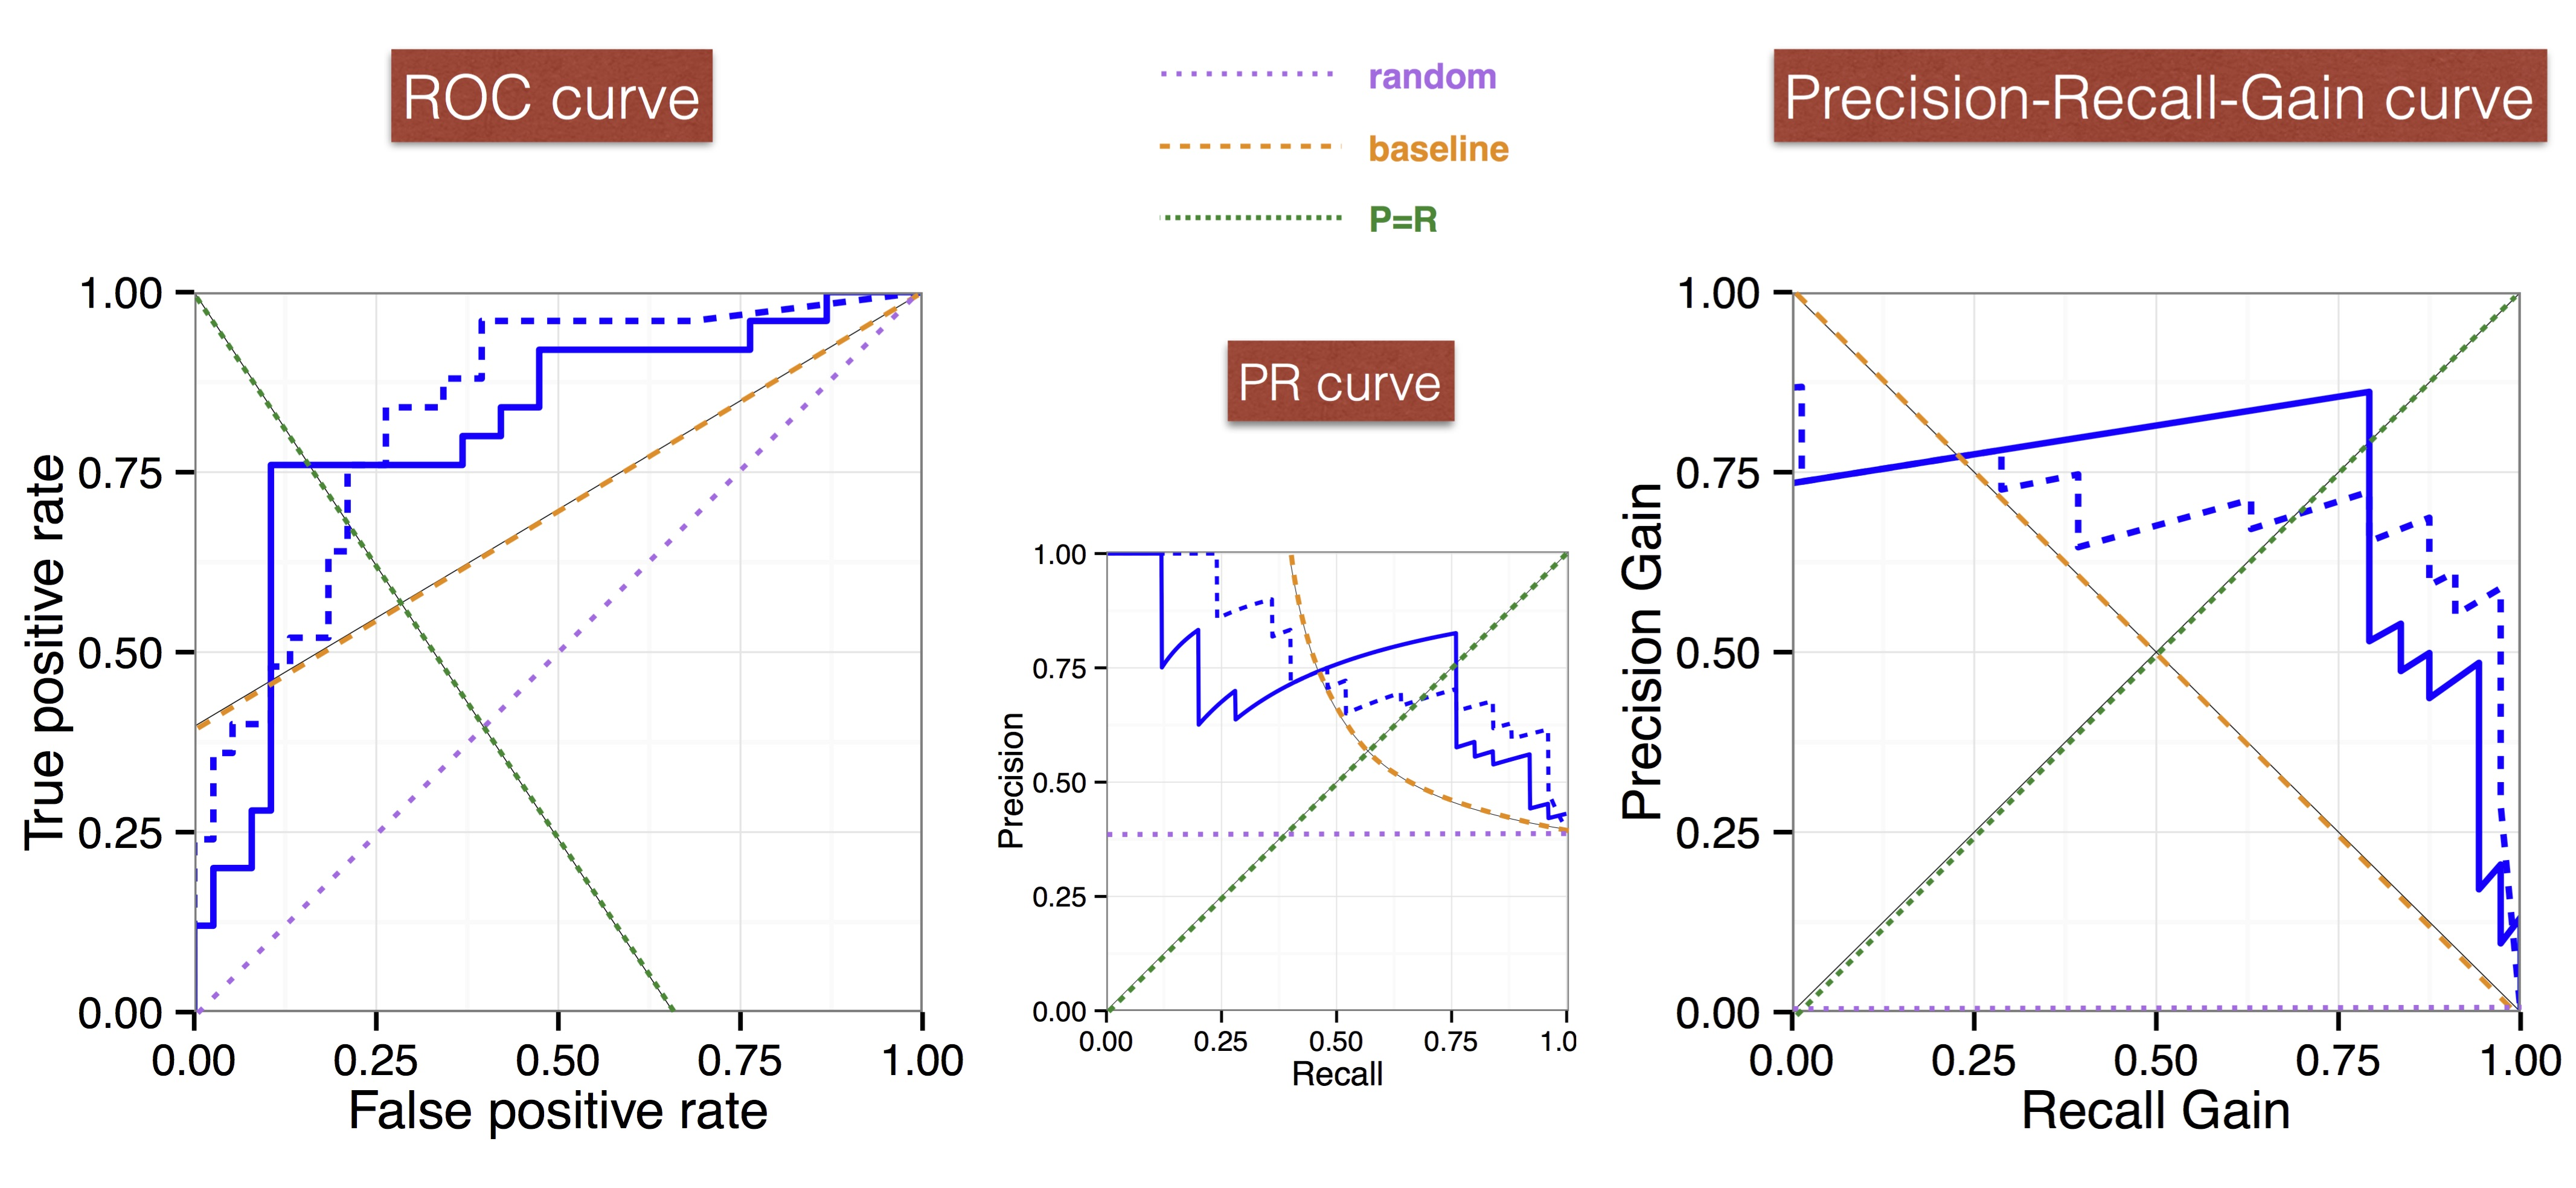
\includegraphics[width=\linewidth]{pediatric-brain-tumours/images/roc-pr-prg-curves.jpg}
    \caption{
        Receiver operating characteristic (ROC) curve, Precision-Recall (PR) curve, and Precision-Recall-Gain curve of two models.
        The random (dotted, purple) and always positive classifier (dashed, yellow) baselines are shown, as well as the $\mathrm{precision} = \mathrm{recall}$ lines.
        The area under the PR curve wrongly suggests that the model with the dashed line performs better, while the area under the PRG curve suggests it's the worst.
        Reproduced from \fullcite{Flach2015} (Ref.~\cite{Flach2015}).
    }
    \label{fig:roc-pr-prg-curve}
\end{figure*}

%%%%%%%%%%%%%%%%%%%%%%%%%%%%%%%%%%%%%

% \subsubsection{Accuracy}

% The accuracy of a binary prediction can be calculated as
% \begin{equation}
%     \text{Accuracy} = \frac{TP + TN}{TP + TN + FP + FN},
% \end{equation}
% where $TP$, $TN$, $FP$, and $FN$ are the number of true/false positive/negative respectively.
% In other words, the accuracy is the number of correct predictions divided by the total number of predictions.

% In the case of imbalanced datasets, accuracy can be misleading.
% \eg if the number of positive samples is much higher than the number of negative samples and a model classifies all samples as positive, the accuracy will be close to one.

% \subsubsection{Informedness}
% Informedness measures the probability of a model giving an informed decision.
% If positive, the model is informed to correctly classify $\mathrm{informedness}\unit{\percent}$ of the time.
% If negative, the model is informed to incorrectly classify $-\mathrm{informedness}\unit{\percent}$ of the time.

% Informedness is calculated as
% \begin{align}
%     \mathrm{informedness} = \mathrm{precision} + \mathrm{recall} - 1,
% \end{align}
% and therefore $\mathrm{informedness} \in [-1, 1]$.

% Informedness may be used to find a prediction probability threshold by maximizing the informedness.

% \subsubsection{$F$-score}

% Another accuracy measure are scores depending on precision and sensitivity (recall).
% The $F_1$-score is the harmonic mean of the precision and recall:
% \begin{equation}
%     F_1 = \frac{2}{\text{recall}^{-1} + \text{precision}^{-1}} = \frac{2 TP}{2 TP + FP + FN}.
% \end{equation}
% In general, $F_\beta$ is a weighted harmonic mean where $\beta\in\mathbb{R}+$, such that recall is $\beta$ times as important as precision:
% \begin{equation}
%     F_\beta = (1+\beta^2)\frac{\text{precision}\cdot\text{recall}}{(\beta^2\cdot\text{precision}+\text{recall})}.
% \end{equation} 

% The $F$-score can take values from 0 (if precision or recall is 0) to 1 (for perfect precision and recall).

% \subsubsection{Area under the precision-recall curve}
% Another performance measure that uses precision and recall is the area under the precision-recall curve (PR-AUC).
% The precision-recall curve (PRC) shows precision and sensitivity pairs at all possible thresholds.
% The higher the PR-AUC, the higher precision and/or recall must be.

% It has been shown that PRC changes with the ratio of positive and negative examples while the receiver operator characteristic curve (another popular performance curve) does not~\cite{Takaya2015}.
% This makes PR-AUC a reasonable choice for imbalanced datasets.

\subsection{Intersection over union}
Image segmentations can be assessed by calculating the intersection over union (IoU) between the segmentation $A$ and a predefined ground truth $B$, as
\begin{align}
    \mathrm{IoU}(A, B) = \frac{|A \cap B|}{|A \cup B|},
\end{align}
where $0 \leq \mathrm{IoU} \leq 1$.
If the segmentation does not intersect the ground truth, then $\mathrm{IoU} = 0$.

